\documentclass[12pt, landscape]{article}
\usepackage[a2paper]{geometry}
\usepackage[numbers]{natbib}
\usepackage{multicol}
\usepackage{blindtext}
\usepackage{setspace}
\usepackage{graphicx}
\usepackage{tikz}
\usepackage{float}
\usepackage{listings}
\usepackage{fancyvrb}
\usepackage{xcolor}

\graphicspath{ {./images/} }
\setlength{\columnsep}{1cm}
\definecolor{beige}{RGB}{250,250,219}
\pagecolor{beige}
%\doublespacing
%\documentclass[12pt,landscape]{article}
%\usepackage[a3paper]{geometry}

\title{Road Sign Recognition with CNN and RCNN}
\author{
  Tahir, Aksel\\
  \texttt{at01053@surrey.ac.uk}
  \and
  Mulvena, Kieran\\
  \texttt{km00220@surrey.ac.uk}
}
\date{11.05.2021}

\begin{document}
\maketitle
%\tableofcontents
%\pagebreak

\begin{multicols}{3}
\section{Introduction}
Road signs are a present system in virtually all road infrastructure. They are
of critical importance to interpreting correct road usage, road regulations and
route recommendations. Their presence is integral to the safe and functional
road use.

Contemporary road signs follow strict design rules to optimise their clarity of
intention. These rules allow them to be as easy as possible for human
interpretation. However, humans are prone to distraction, misinterpretation and
other general mistakes, which is why road sign recognition (RSR) algorithms are
a fast-advancing point of development in autonomous driving research.

Standard computer vision methods are not versatile enough to deal with the
plethora of different physical road conditions. This is why applying a deep
learning approach to the problem is necessary - A well crafted AI can exceed
even human vision in RSR.

In this project we propose an RSR solution using several different neural
network models and evaluating their performance. Since standard computer vision
methods are not versatile enough to deal with the plethora of different physical
road conditions, it is necessary to apply a deep learning approach to the
problem - A well crafted AI can exceed even human vision in RSR.

\section{Related Work}
With the advent of AI computing autonomous and assisted driving has been an area
of extensive research. Road sign recognition (RSR) systems are integral to the
field. The functional implementation of RSR systems depends on two related
issues - Road sign detection (RSD) and road sign classification (RSC). RSD
pertains to localising the relevant information from the data, and RSC to
identifying the data with its correct labels. There have already been a number
of outstanding studies in the detection and classification in
\citep{Classification1}, \citep{Classification2}, \citep{Classification3},
\citep{Classification4}, \citep{Classification5}.

In many RSR systems, the RSD part is done via conventional machine learning
methods. This approach is used by authors like Amal Bouti et al in
\citep{Recognition1}. The advantages of deep learning methods have made
themselves clear by now, but the author has chosen to discuss if SVMs do not still
have a place in RSR. In their findings, "the representation of the HOG features
and SVM greatly improves the results obtained and shows good results in terms of
accuracy. The linear SVM not only achieves high accuracy but also costs least
compared with another kernel function" \citep[6722 A. Bouti et al]{Recognition1}

[Add info about R-CNN too. That'd be pretty useful]

\section{Architectures}
This project is based entirely on image recognition, the models we have decided
to implement are all CNN-based. This section will describe them all in detail.

\subsection{CNN}
Recent decades have seen many advancements in representational learning from raw
data, with one of the most pertinent approaches to the method being the
varieties of CNN modelling. CNN dominates systems related to object recognition
and detection. This ubiquity in the field is one of the reasons that made us
choose it for our implementation.

Another major advantage of CNNs that led to our choice is the relatively sparse
pre-processing required to make a functioning model, compared to more
traditional image classifiers. The independent kernel optimisation that CNNs
learn, without much prior knowledge is hugely beneficial to implementation
complexity.

We have decided to implement two different CNN classifiers parallel to
each other, with the intention of seeing if our approaches and results will have
any significant differences. Aksel's CNN implementation will be referred to as
(CNN-A) and Kieran's as (CNN-K).

\subsection{R-CNN}
At the time of writing the R-CNN model has not been implemented.

\subsection{Faster R-CNN}
At the time of writing the Faster-R-CNN model has not been implemented.

\section{Dataset}
This project intends to use two datasets to conduct its study to ensure
flexibility and better insight. The data needed for detection differs from that
needed for classification, and many datasets do not meet both requirements. This
section will discuss our choices and their features.
\subsection{GTSRB - German Traffic Sign Recognition Benchmark}
The German Traffic Sign Recognition Benchmark is our first choice. It contains
43 data classes of road signs in Germany with each having enough examples to be
used in training.

\begin{itemize}
    \item As seen from the examples in Figure~\ref{fig:dataset1examples} dataset
    is only useful for classification purposes and not detection, since its
    items only feature photos of isolated road signs with no irrelevant data in
    the image.
    \begin{figure}[H]
        \centering
        \begin{tabular}{cc}
        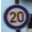
\includegraphics[scale=1.3]{ex1.png}&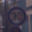
\includegraphics[scale=1.3]{ex2.png}\\
        
\includegraphics[scale=1.3]{ex3.png}&
\includegraphics[scale=1.3]{ex4.png}\\
        \end{tabular}
        \caption{Some examples of raw data from the dataset}
        \label{fig:dataset1examples}
    \end{figure}

    \item The dataset also contains unequal numbers of items in each class, as
    seen in Figure~\ref{fig:dataset1balance}, which introduces a challenge solved in
    Preprocessing.
    \begin{figure}[H]
        \centerline{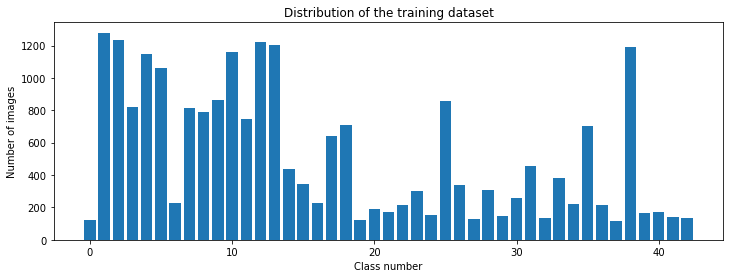
\includegraphics[scale = 0.5]{download.png}}
        \caption{Number of items in each class of GTSRB}
        \label{fig:dataset1balance}
    \end{figure}

  \end{itemize}

\subsubsection{Loading the dataset}
The ~50K images loaded from the dataset were split into two groups for training
and testing. The split was arbitrarily chosen to be 0.8/0.2 respectively. Out of
the 80\% chosen for training, 20\% were chosen for validation.

\color{red}
\begin{Verbatim}[fontsize=\small]
1   testRatio = 0.2 
2   # set aside 20% of images for testing, 80% for training
3   validationRatio = 0.2 
4   # of all training images, set aside 20% for validation
5
6   X_train, X_test, y_train, y_test = 
7   train_test_split(images, classNo, test_size=testRatio)
8   X_train, X_validation, y_train, y_validation = 
9   train_test_split(X_train, y_train, test_size=validationRatio)
10 
11  # X_train = ARRAY OF IMAGES TO TRAIN
12  # y_train = CORRESPONDING CLASS ID
\end{Verbatim}
\color{black}

\subsubsection{Preprocessing data}
There are quite a few tasks to be done with preprocessing the data from this
dataset. 

\paragraph{Dataset Balancing}
Data imbalance reflects an unequal distribution of classes within the dataset,
as we can see in Figure~\ref{fig:dataset1balance}. This disproportion needs to
be leveled out for better classification. We do this with two techniques -
\emph{undersampling} and \emph{oversampling}

Since we have such a huge imbalance in class values, using either an
undersampling or oversampling algorithm would not work well. This is why we take
a more nuanced approach of using both algorithms to make an augmented dataset
with values meeting somewhere in the middle of both extremes.
\begin{figure}[H]
    \centerline{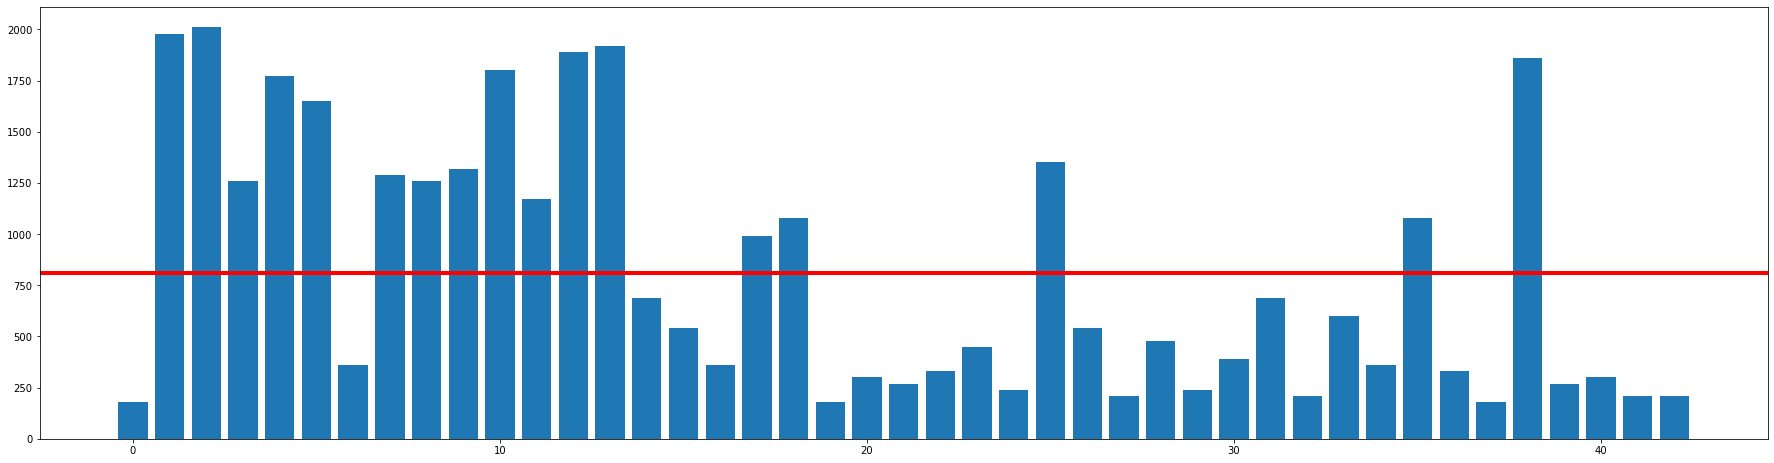
\includegraphics[scale = 0.2]{classbalance.png}}
    \caption{Class balance point}
    \label{fig:dataset1balancemid}
\end{figure}
Figure~\ref{fig:dataset1balancemid} shows a close approximation of the average value
each class should achieve. Accordingly, we oversample the ones below the line
and undersample the ones above it.

To undersample, we simply take random values from the larger classes and remove
them until they reach the midpoint.

To oversample, we are trying out a few different algorithms. SMOTE is one of
them, which synthesizes new examples for the minority classes. As described by
\citep[Nitesh Chawla et al]{SMOTE} in their paper, SMOTE works by selecting
examples that are close in the feature space, drawing a line between the
examples in it and drawing a new sample at a point along that
line.


\paragraph{Image Augmentation}
In CNN-A, the images are augmented - They are converted to a
monochromatic greyscale and then undergo histogram equalisation. Finally
their values are normalised from 0-255 to 0-1.

Other augmentations the team has considered is using synthetic noise addition in
order to test the accuracy of the model against more obscured data, simulating
real life conditions such as rain and mist, but as of writing this
implementation has not been completed.


\subsection{GTSDB - German Traffic Sign Detection Benchmark}
The previous dataset was very useful for RSC, but it did not contain the needed
info for RSD. This is why we're also incorporating the GTSDB for our study into
detection. It contains images of german roads with visible road signs which take
up a fraction of the image itself.
\begin{figure}[H]
    \centering
    \begin{tabular}{cc}
    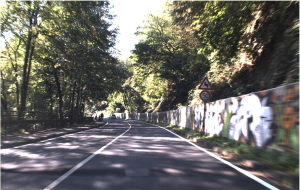
\includegraphics[scale=0.5]{example1.png}&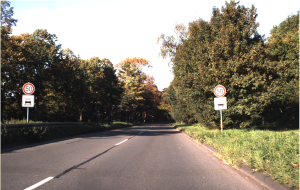
\includegraphics[scale=0.5]{example2.png}\\
    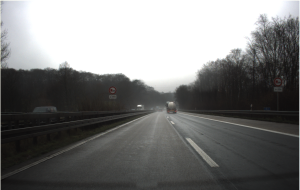
\includegraphics[scale=0.5]{example4.png}&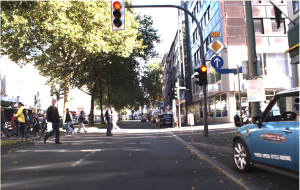
\includegraphics[scale=0.5]{example3.png}\\
    \end{tabular}
    \caption{Some examples of raw data from the dataset}
    \label{fig:dataset2examples}
\end{figure}
\begin{itemize}
    \item The dataset contains 900 separate images
    \item The images contain zero to six traffic signs
    \item The sizes of the traffic signs in the images vary from 16x16 to 128x128
    \item Traffic signs may appear in every perspective and under every lighting
    condition
\end{itemize}

Like GTSRB, this dataset also has 43 classes (or 44 when counting the background as a class) with an imbalance in numbers.
\begin{figure}[H]
    \centerline{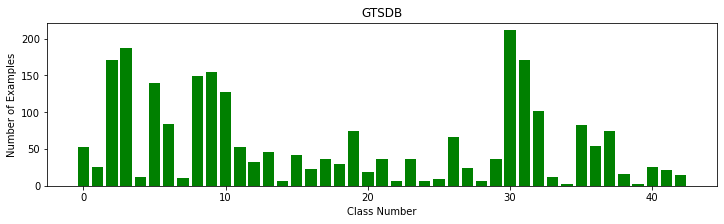
\includegraphics[scale = 0.5]{gtsdb.png}}
    \caption{Class balance point}
    \label{fig:dataset2balance}
\end{figure}


\section{Implementation}

\subsection{CNN-A}
Modelling this CNN is very straightforward with Keras. The model we've chosen the
CNN-A implementation closely resembles LeNet (Figure~\ref{fig:lenetstructure}),
proposed by Yann LeCun et al in 1998. The dataset we've trained the model upon
is the GTSRB.
\begin{figure}[H]
    \centerline{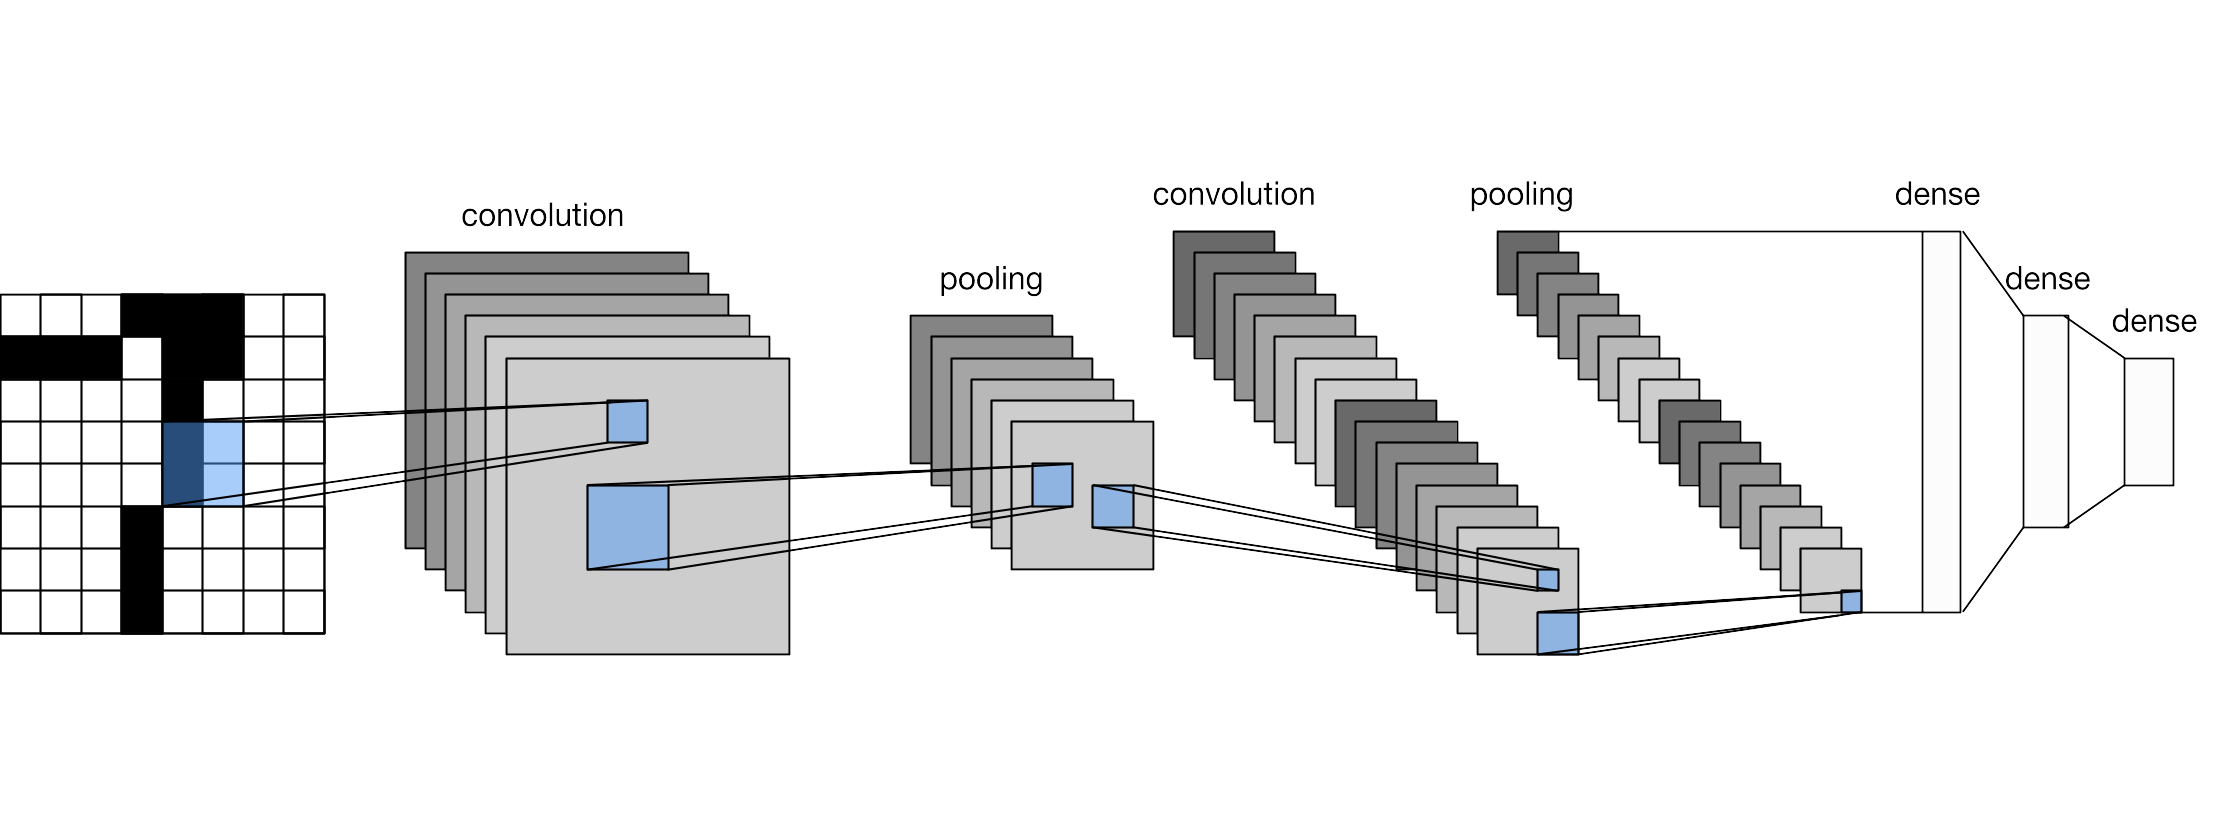
\includegraphics[scale = 0.2]{lenet.png}}
    \caption{Generic LeNet structure}
    \label{fig:lenetstructure}
\end{figure}

\subsubsection{Structure}
\begin{figure}[H]
    \centerline{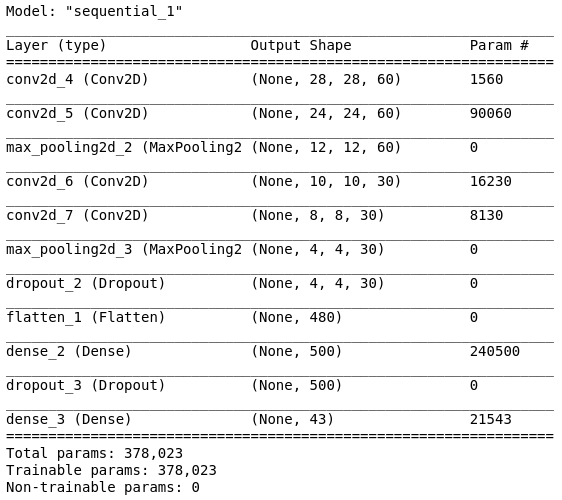
\includegraphics[scale = 0.5]{model.png}}
    \caption{Structure of our CNN-A model}
    \label{fig:CNNAstructure}
\end{figure}

The first two layers are convolutions. Layer 1 has a depth of 60, a filter size
of (5, 5), with relu activation. The second layer does the same. Following the
second convolution layer is a max polling layer. Following the LeNet model, we
use a (2,2) kernel size. It effectively downsizes the data by only selecting the
max value pixel for adjacent pixels.

Next we implement two other convolution layers with new parameters. Half the
number of filters and a filter size of (3,3). Their activation is also relu.
They're followed by a max pooling layer and a dropout layer to prevent
overfitting the model. 

Afterwards, the data is flattened and a dense layer with relu activation is
used. A second dropout layer prepares the model for the a last fully connected
dense layer with class number as size (ie. 43). Softmax is used to return the
probabilities of each class, and the model is compiled with the Adam optimiser.

\subsubsection{Performance and Results}
\begin{figure}[H]
    \centering
    \begin{tabular}{cc}
    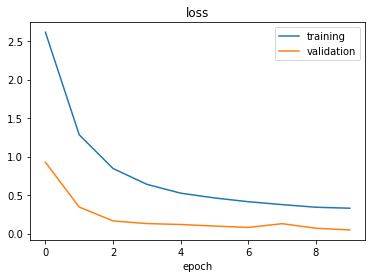
\includegraphics[scale=0.45]{accuracy1.png}&
    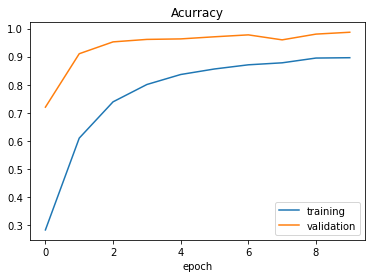
\includegraphics[scale=0.45]{accuracy2.png}\\
    \end{tabular}
    \caption{The Loss and Accuracy values throughout the epochs}
    \label{fig:CNNAaccuracy}
\end{figure}
Within 10 epochs, the accuracy of both training and validation is above 0.98,
after which the model shows minimal improvements and the cost/ gain balance
becomes unreasonable.

This model achieved formidable results with relatively light training. After
roughly 30 minutes on Heron labs computers and 10 epochs the test accuracy
averaged in the 98th percentile. Figure~\ref{fig:CNNAaccuracy} shows the
relevant values throughout training

\begin{figure}[H]
    \centerline{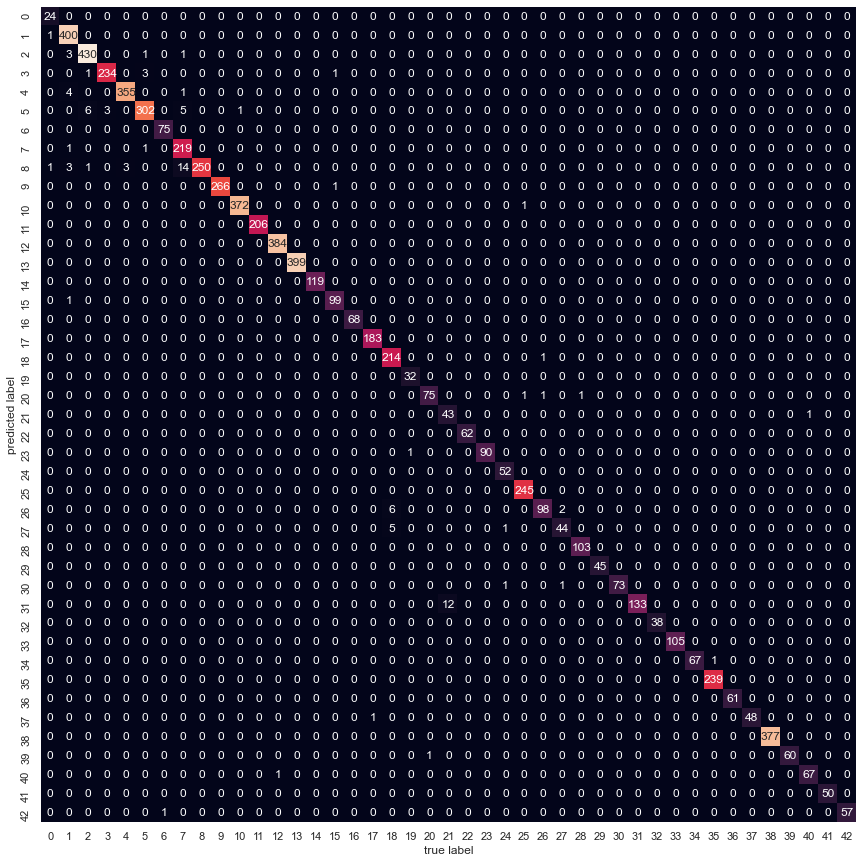
\includegraphics[scale = 0.4]{confmat.png}}
    \caption{Confusion Matrix for CNN-A}
    \label{fig:CNNAconusionmatrix}
\end{figure}
\begin{figure}[H]
    \centerline{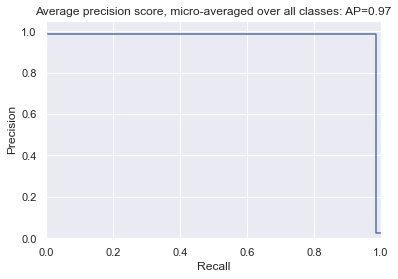
\includegraphics[scale = 0.6]{precisionrecall.png}}
    \caption{Precision and recall plot}
    \label{fig:CNNAprecrec}
\end{figure}

\begin{center}
\emph{Accuracy(true values, predicted values) $\approx$ 0.99}

\emph{Average precision score, micro-averaged over all classes $\approx$ 0.97}
\end{center}


\subsection{CNN-K}
Along with the difference in preprocessing, this implementation uses a different
model structure than the one in CNN-A. CNN-K studies two models, but in this
poster we will only look at the one reaching better results for the sake of
being concise.

\subsubsection{Structure}
\begin{figure}[H]
    \centerline{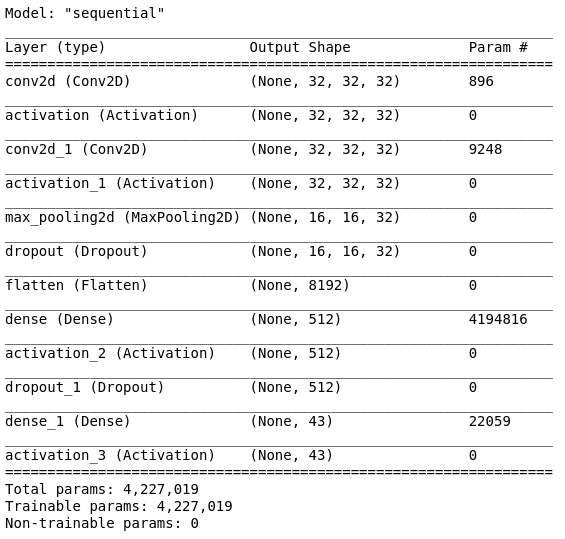
\includegraphics[scale = 0.5]{figuremodel1.png}}
    \caption{Structure of our CNN-K model}
    \label{fig:CNNKstructure}
\end{figure}
Unlike the CNN-A implementation, this one begins with a convolutional layer of a
32,32,32 shape. An activation layer preceeds the second convolution. There is a
second activation, after which the data is reshaped in a max pooling grid.

It undergoes dropout and flattening, and the 8th layer is the first dense layer.
Another activation and dropout later, the data passes through the final dense
and activation layers and the output shape is 43, denoting the classes.

\subsubsection{Performance and Results}
\begin{figure}[H]
    \centering
    \begin{tabular}{cc}
    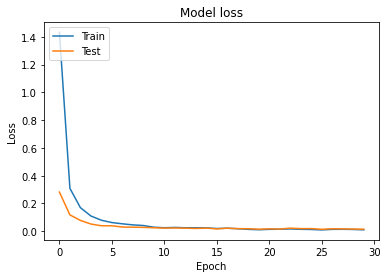
\includegraphics[scale=0.45]{Kresult1.png}&
    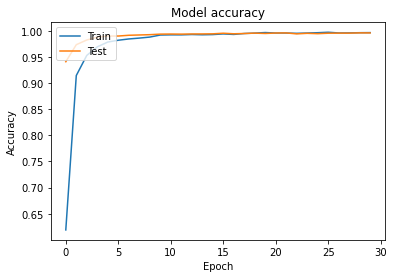
\includegraphics[scale=0.45]{Kresult.png}\\
    \end{tabular}
    \caption{The Loss and Accuracy values throughout the epochs}
    \label{fig:CNNKaccuracy}
\end{figure}
The model is fitted with 30 epochs, but as with the previous implementation, the
accuracy of both training and validation is above 0.98, after which the model
shows minimal improvements and the cost/gain balance becomes unreasonable.

\subsection{Faster R-CNN}
The Faster R-CNN of our project is based on the implementation found at the
open-source repository by github user \citep[Haxothermic]{Haxothermic}. 
\subsubsection{Augmentation}
Running the source code is straightforward after installing the needed libraries
and adapting it to our dataset. We begin with data loading and augmentation. The
latter is done with the built-in transform functions in PyTorch. The augmented
results are shown in Figure~\ref{fig:RCNNaugmentation}. 

\begin{figure}[H]
    \centering
    \begin{tabular}{cc}
    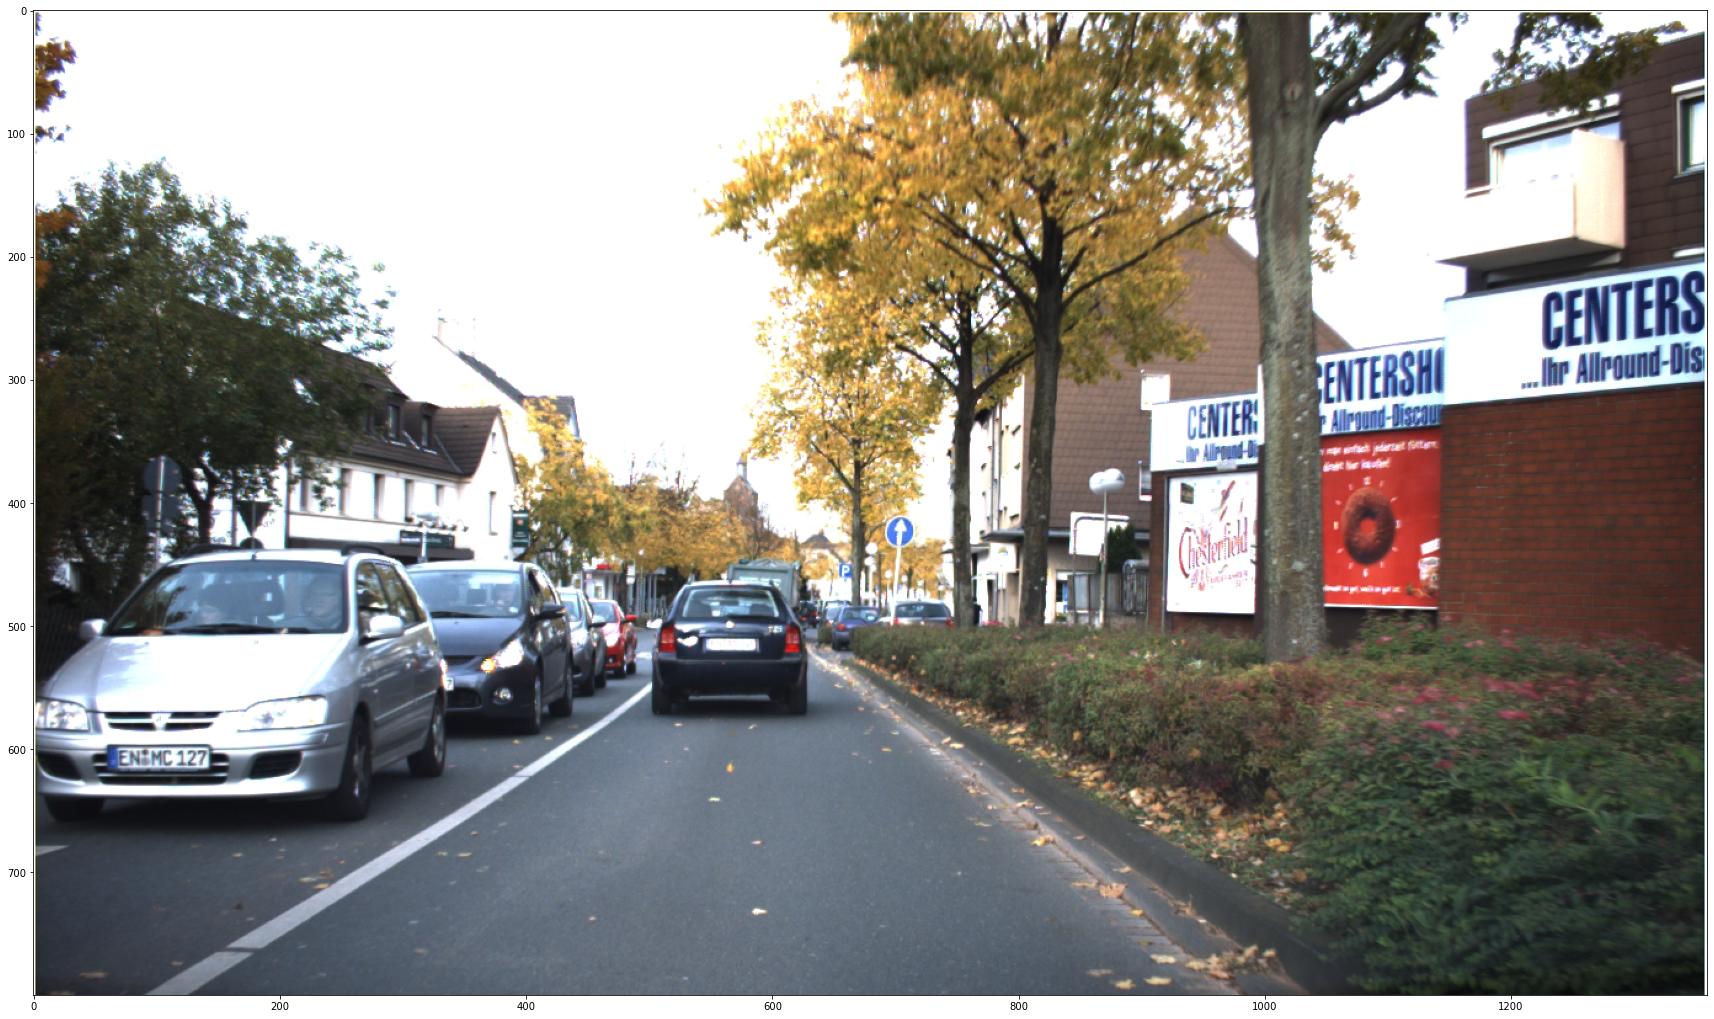
\includegraphics[scale=0.105]{rcnnimg2.png}&
    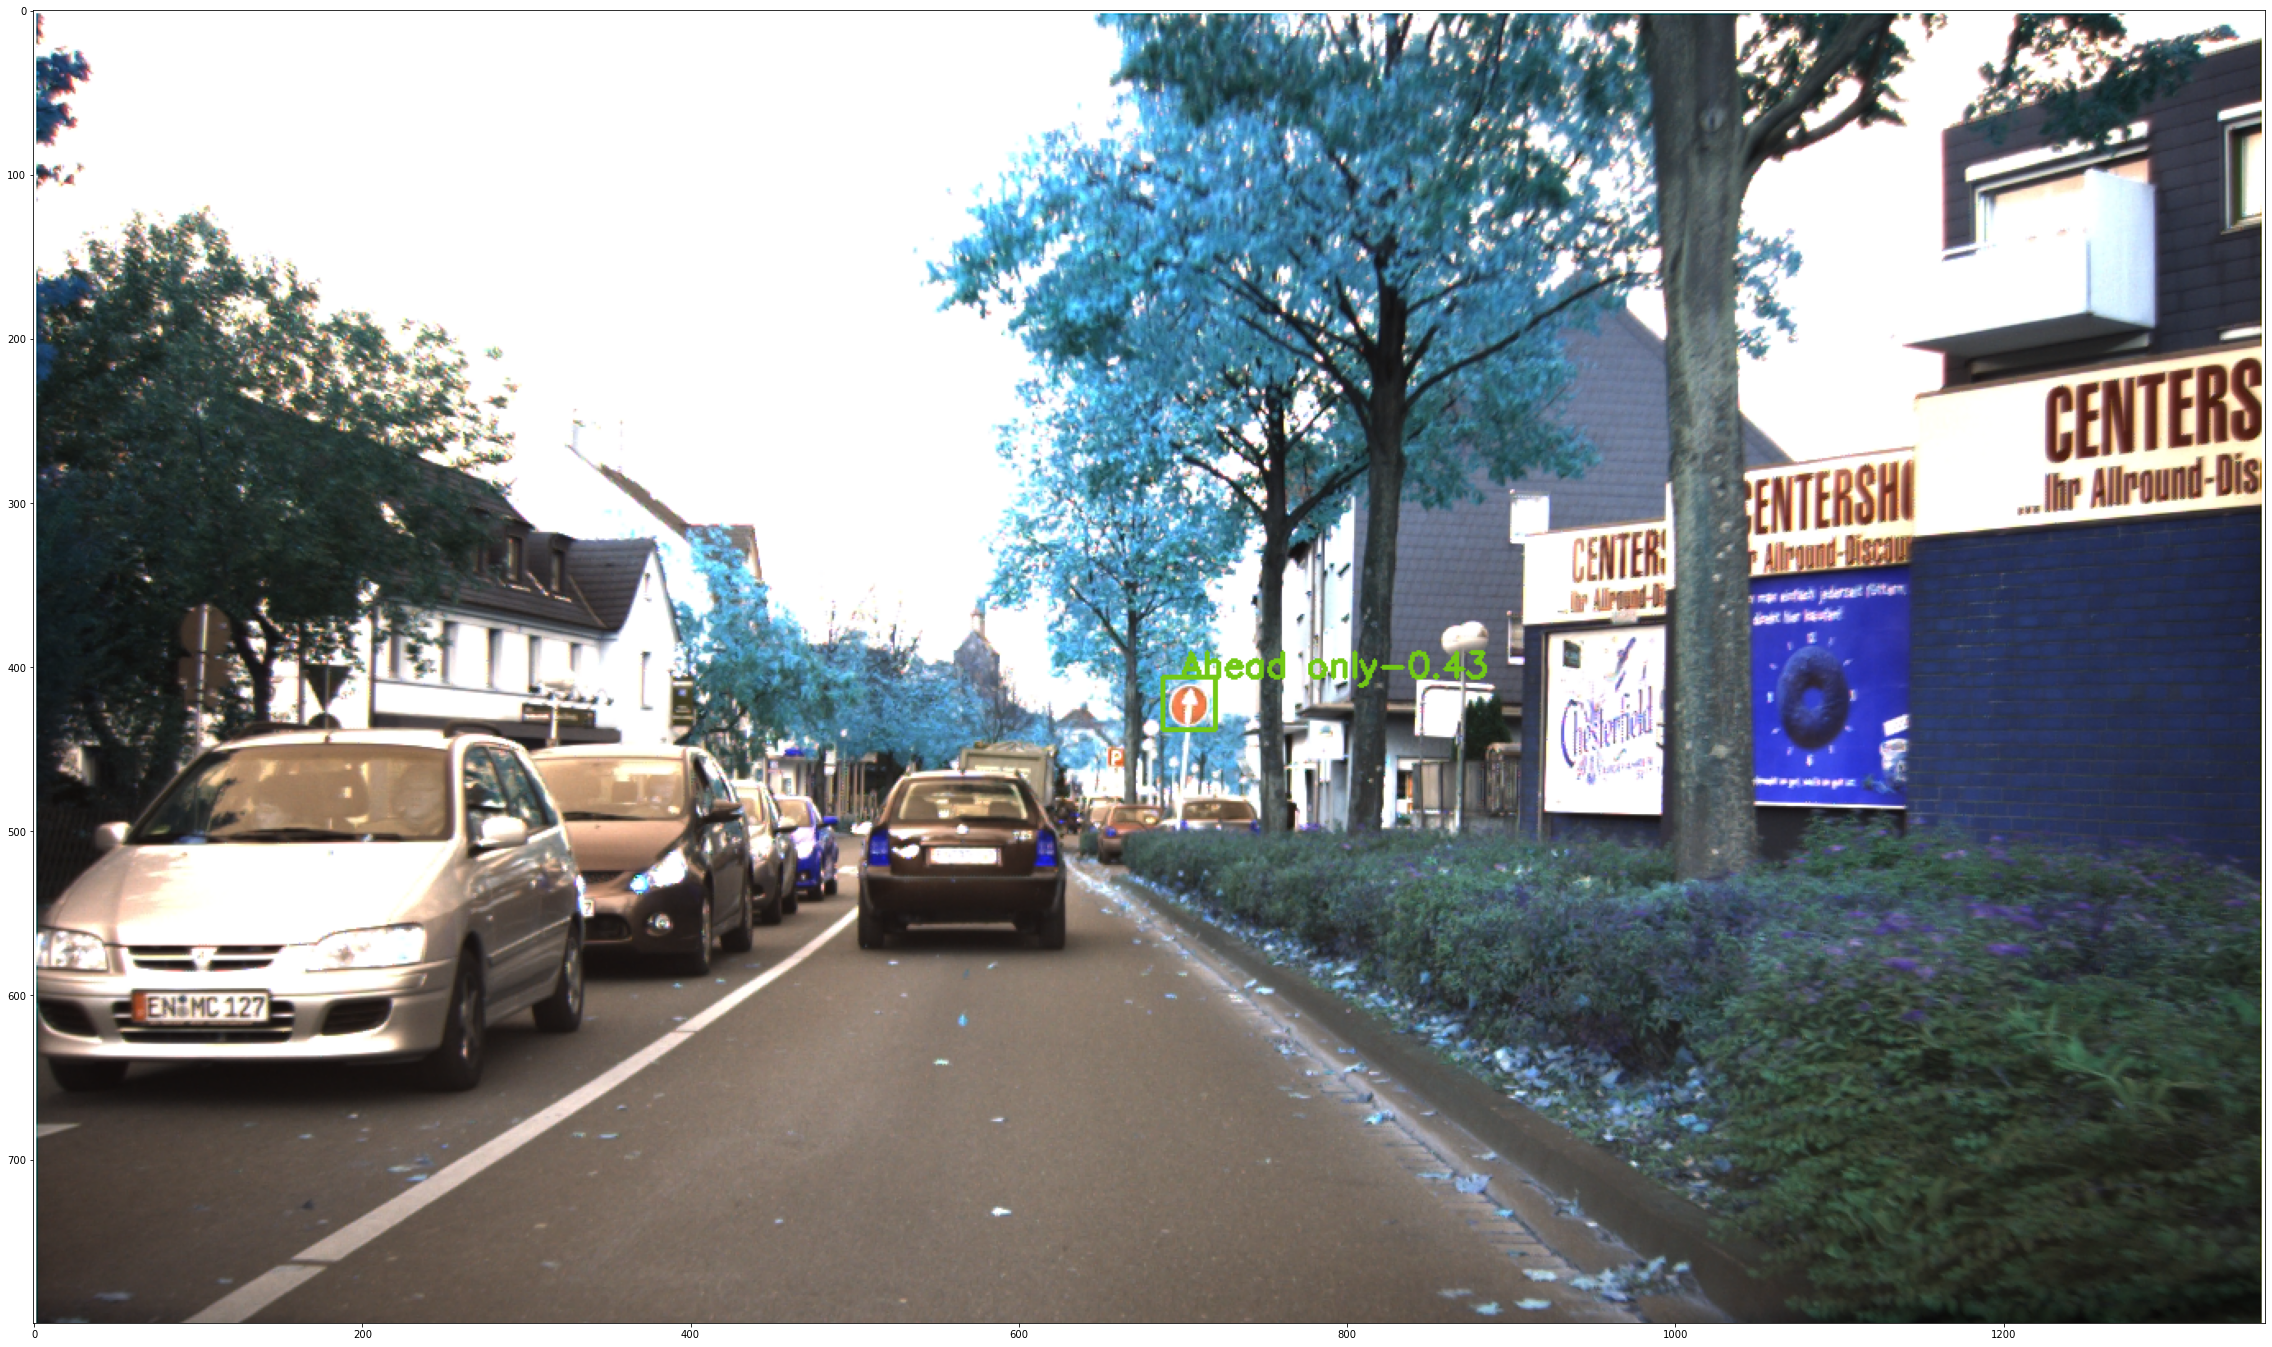
\includegraphics[scale=0.08]{rcnnimg1.png}\\
    \end{tabular}
    \caption{The image before and after augmentation via the PyTorch functions}
    \label{fig:RCNNaugmentation}
\end{figure}

\subsubsection{Defining model and loading data}
\begin{itemize}
    \item We declare the train and test datasets by calling the myDataset class
    which was defined earlier.
    \item Afterwards, we split the dataset into two 4:1 Train to Test approximately.
    \item Using PyTorch's DataLoader to load data.
    \item Defining the model - Faster RCNN with a pretrained ResNet50 backbone
    network is used to finetune according to our dataset.
    \item Defining all the parameters required for training. (Using SGD as
    optimizer, Cosine Annealing/Decreasing Warm Restarts as learning rate
    scheduler which decreases the initial learning rate set in a cosine manner
    until a restart; the lr is set back to the initial lr and the cycle repeats,
    number of epochs = 1000)
    \item Declaring all the variable to be retrieved from the COCO Evaluation
    metrics.
    \item We start training the model and then evaluate the performance on test
    set.
\end{itemize}

\subsubsection{Performance and Results}
To discuss the performance we must first set some terminology:
\begin{itemize}
    \item \emph{True Positive \textbf{(TP)}} - Results where the Intersection
    Over Union (IOU) over the predicted bounding box and ground truth is at
    least equal to the threshold.

    \[\frac{Intersection Over Union}{Predicted Ground Box+Ground Truth} \geq
    Threshold\]

    \item \emph{False Positive \textbf{(FP)}}

    \[\frac{Intersection Over Union}{Predicted Ground Box+Ground Truth} <
    Threshold\]

    \item \emph{Average Precision \textbf{(AP)}} - The number of true positives
    in the resulting bounding boxes.

    \item \emph{Average Recall \textbf{(AR)}} - The proportion of true positives
    out of possible positives.
\end{itemize}

The following can be inferred from the stats of the last iteration:
\begin{itemize}
    \item The AP at IoU = 0.5-0.95 for large areas is 0.800 which means that when
    the model detects an object with large area, 80\% of the time it matches the
    ground truth objects.

    \item The AR  at IoU = 0.5-0.95 for large is 0.800 which means that the
    model detects 80\% of objects with large area, correctly.

    \item For medium and small areas, the model does not do well. This is
    probably caused by the size of the dataset and the insufficient number of
    examples for small and medium sized objects.
\end{itemize}

\begin{figure}[H]
    \centerline{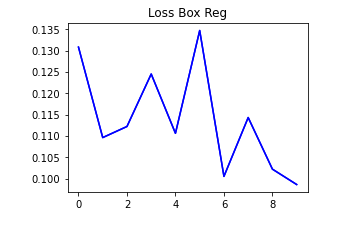
\includegraphics[scale = 0.6]{lossboxreg.png}}
    \caption{Loss Box Reg - The measure of how tightly the model predicted the bounding box around the true object. It can be observed that the model works well to fit the bbox tightly to the object.}
    \label{fig:LosBoxReg}
\end{figure}

\begin{figure}[H]
    \centerline{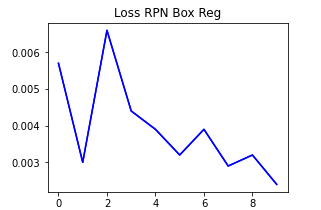
\includegraphics[scale = 0.6]{lossrpnboxreg.png}}
    \caption{Loss RPN Box Reg - This measures the performance of the network for retrieving the region proposals. The plot shows that further training or tweaking the hyperparameters may be required to decrease the loss. This may require more data to improve the results significantly.}
    \label{fig:LossRPNBoxReg}
\end{figure}

\begin{figure}[H]
    \centerline{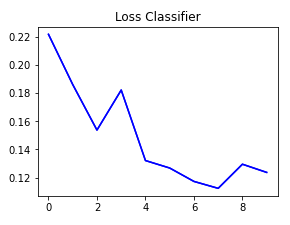
\includegraphics[scale = 0.6]{lossclassifier.png}}
    \caption{Loss Classifier - This measures the performance of the object classification for detected bounding boxes. The plot shows that the model performs well in classifying the objects in the detected bounding boxes.}
    \label{fig:LossClassifier}
\end{figure}

\begin{figure}[H]
    \centerline{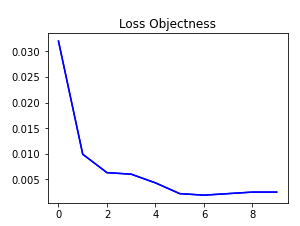
\includegraphics[scale = 0.6]{lossobjectness.png}}
    \caption{Loss Objectness - This measures the performance of network for retrieving bounding boxes which contain an object. We can infer that the model is detecting the object very well.}
    \label{fig:LossObjectness}
\end{figure}

\section{Conclusions}
%data goes in and numbers come out and we don't question any of it

In this project we tried to propose a road sign recognition system with two
distinct phases - Classification and Detection. For the classification phase we
adapted a LeNet CNN model and another CNN model with highly successful results.
For our detection phase we used an RCNN model with some room for future
improvement. We used the german road sign datasets for classification and
detection, both of which had to undergo some preprocessing to achieve good
results.

Our concluding observations are that using CNN and RCNN technologies remains an
incredibly robust option for any recognition software, and has many potential
real-life uses given the right development and optimisation.

Future work may include using different datasets to expand the model with more
classes and examples, fine-tuning our RCNN model for better detection,
implementing more variants of RCNN, fusing our CNN and RCNN implementations into
one, etc. The topic at hand is incredibly rich with opportunity, so it is only a
matter of time.
\bibliographystyle{unsrt}
\bibliography{References}
% \nocite{*}
\end{multicols}
\end{document}